\exercise{Zooming and shrinking by bilinear interpolation}
\subsection*{a - \texttt{IPresizebl}}
For this exercise, a \textit{MATLAB} function was made that is able to rescale an image.
The pixels of the rescaled image have to be interpolated in the original image, using bilinear interpolation.
This means that we look at the four pixels in the original image that are closest to the required position, and take the weighted average of those.

The code is given and explained below:
\matlabexternal{IPresizebl.m}

The function takes a scaling factor for the x-direction ($x_f$) and y-direction($y_f$). Then for each sampling point the four nearest pixels in the original image are stored. The sampled value in the scaled image is the bilinear interpolation of the values of the neighboring pixels of the sampling point.
\subsection*{b - Resizing a chronometer}
The file \texttt{chronometer1250dpi.tif} is an image file of a very high resolution.
For some purposes it is useful to have a smaller images.
Our function, \texttt{IPresizebl} is made for exactly this purpose.

For comparison, the original image of the chronometer is shown in Figure~\ref{fig:chrono_original0}.
The image that is downscaled with a factor 12.5 is shown in Figure~\ref{fig:chrono_down}.

\begin{figure}[!Htb]
 \centering
 \includegraphics{originalChrono.eps}
 \caption{Original chronometer image.}
 \label{fig:chrono_original0}
\end{figure}

\begin{figure}[!Htb]
 \centering
 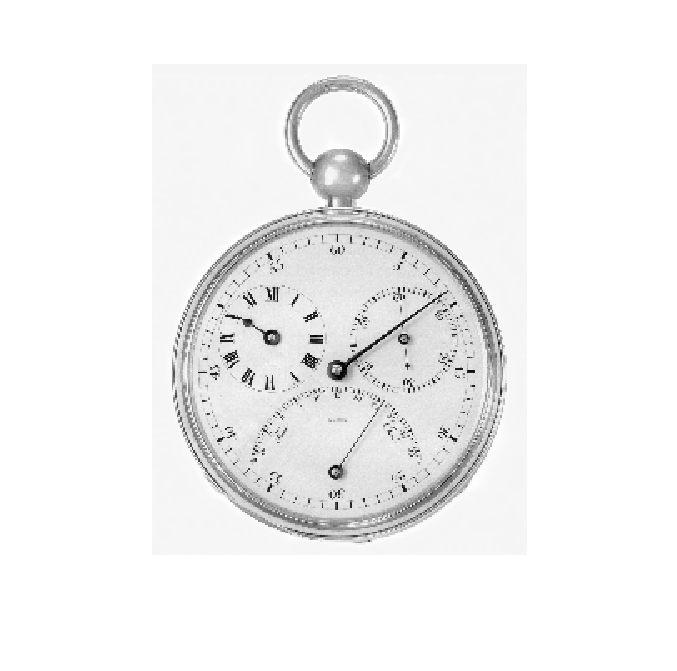
\includegraphics{scaledDownChrono.eps}
 \caption{Downscaled chronometer by a factor 12.5. An artifact of downscaling is the `pixelization' of the image.}
 \label{fig:chrono_down}
\end{figure}

\clearpage

\subsection*{c - Upscaling a downscaled chronometer}
Of course, after downscaling, information is lost. This can be visualized by scaling the downscaled image back up to the original size, and comparing the result to the original image. The comparison is shown in Figure \ref{fig:chrono_compare}. It is clear that figure~\ref{fig:chrono_original0} is not equal to figure~\ref{fig:chrono_compare}. It is especially promiment at the edges of the rescaled images. Here noticable artifacts are introduced in the image which are the result of information loss in the downsampling step. 

\begin{figure}[!Hbt]
\centering
 \begin{subfigure}[b]{0.45\textwidth}
  \includegraphics[width=\textwidth]{originalChrono.eps}
  \caption{Original chronometer}
  \label{fig:chrono_original1}
 \end{subfigure}
 \begin{subfigure}[b]{0.45\textwidth}
  \includegraphics[width=\textwidth]{rescaledUpChrono.eps}
  \caption{Re-upscaled chronometer}
  \label{fig:chrono_down_up}
 \end{subfigure}
 \caption{Comparation of original chronometer and the downscaled chronometer that has been upscaled back to the original size. During the downscaling, only the weighted averages of four pixels are stored, so the original information is lost. Moreover, not even all pixels in the original image always contribute to the downscaled image, since some pixels are simply skipped.}
 \label{fig:chrono_compare}
\end{figure}

\clearpage